\documentclass[12pt, a4paper, oneside]{ctexart}
\usepackage{listings}
\usepackage{tikz}
\usepackage{amssymb}
\usepackage{t-angles}
\usepackage{amssymb}
\usepackage{tikz}
\usepackage{mathrsfs}
\usepackage{pifont}
\usepackage{amsmath}
\usepackage{fixdif}
\usepackage{mathrsfs}
\usepackage{pdfpages}
\usepackage[bookmarks=true, colorlinks, citecolor=blue, linkcolor=black]{hyperref}
\newcommand{\E}{\mathscr{E}}
% 导言区

\title{电磁学期末复习讲义}
\author{曳涂}
\date{\today}

\begin{document}

\maketitle
\begin{center}
    \begin{figure}[htbp]
       \centerline{ \includegraphics*{dfx6sr6m.png}}
    \end{figure}
\end{center}
\newpage

\tableofcontents
\newpage
\section{数学预备}
以下公式均不做证明
$$\begin{aligned}
    \vec{A}\times(\vec{B}\times\vec{C})&=(\vec{A}\cdot\vec{C})\vec{B}-(\vec{A}\cdot\vec{B})\vec{C}
\end{aligned}$$
在直角坐标中:
$$\begin{aligned}
\nabla f&=\frac{\partial f}{\partial x}\hat{x}+\frac{\partial f}{\partial y}\hat{y}+\frac{\partial f}{\partial z}\hat{z}\\
\nabla \cdot \mathbf{a}&=\frac{\partial a_x}{\partial x}+\frac{\partial a_y}{\partial y}+\frac{\partial a_z}{\partial z}\\
\nabla \times \mathbf{a}&=(\frac{\partial a_z}{\partial y}-\frac{\partial a_y}{\partial z})\hat{x}+(\frac{\partial a_x}{\partial z}-\frac{\partial a_z}{\partial x})\hat{y}+(\frac{\partial a_y}{\partial x}-\frac{\partial a_x}{\partial y})\hat{z}\\
\nabla^2f&=\frac{\partial^2 f}{\partial x^2}+\frac{\partial^2 f}{\partial y^2}+\frac{\partial^2 f}{\partial z^2}
\end{aligned}$$
柱坐标:
$$\nabla f=\frac{\partial f}{\partial r}\hat{r}+\frac{\partial f}{r\partial\theta}\hat{\theta}+\frac{\partial f}{\partial z}\hat{z}$$
球坐标:
$$\nabla f=\frac{\partial f}{\partial r}\hat{r}+\frac{\partial f}{r\partial\theta}\hat{\theta}+\frac{\partial f}{r\sin\theta\partial \phi}\hat{\phi}$$
\newpage
\section{公式集锦及知识点梳理}
\subsection{静电场及电介质}
\subsubsection{静电场基本物理量}
库伦定律
$$\vec{F}=\frac{1}{4\pi\varepsilon_0}\frac{q_1q_2}{r^2}\hat{r}$$
$$\vec{E}=\frac{\vec{F}}{q}$$
由库伦定律可导出高斯定理
$$\oint \vec{E}\cdot \d \vec{S}=\sum\frac{q}{\varepsilon_0}$$
微分形式为
$$\nabla\cdot\vec{E}=\frac{\rho}{\varepsilon_0}$$
静电场的环路定理
$$\oint\vec{E}\cdot\d \vec{l}=0$$
微分形式为
$$\nabla\times\vec{E}=0$$
由环路定理,我们可以将$\vec{E}$写为某个势函数的梯度,定义电势函数$\varphi$
使得
$$\vec{E}=-\nabla\varphi$$
$\varphi$的零点原则上是任取的,但是为了方便通常取在无限远处(某些无穷远处
有电荷分布的情况较为特殊)。无穷远处为势能零点时,某一点电势定义为
$$\varphi_A=U_{A\infty}=\int_A^\infty \vec{E}\cdot\d \vec{l}$$
\subsubsection{电偶极子}
电偶极子由两个等量异种电荷组成,是一个点模型,其特征由电偶极矩刻画
$$\vec{p}=q\vec{l}$$
$\vec{l}$是由负电荷中心指向正电荷中心的矢量。电偶极子在空间某点产生的
电势及场强为
$$\begin{aligned}
    V(\vec{r})&=\frac{1}{4\pi\varepsilon_0}\frac{\vec{p}\cdot\vec{r}}{r^3}\\
    \vec{E}(\vec{r})&=\frac{1}{4\pi\varepsilon_0r^5}[3(\vec{p}\cdot\vec{r})\vec{r}-r^2\vec{p}]
\end{aligned}$$
电偶极子在外电场中电势能,所受合力及力矩为
$$\begin{aligned}
    W&=-\vec{p}\cdot\vec{E}\\
    \vec{F}&=\nabla(\vec{p}\cdot\vec{E})\\
    \vec{L}&=\vec{p}\times\vec{E}
\end{aligned}$$
\subsubsection{导体}
在外电场中导体内部电荷会受到电场力作用从而重新进行分配,使得导体内部电场为0,整个导体成为
等势体,电荷分布在导体表面。电荷面密度为
$$\sigma=\varepsilon_0E$$
\subsubsection{相互作用能}
$$W=\frac{1}{2}\iiint \rho U\d V=\frac{1}{2}\iiint\vec{E}\cdot\vec{D}\d V$$
\subsubsection{电容}
$$C\equiv \frac{q}{U}$$
电容器所带能量为
$$\frac{QU}{2}=\frac{CU^2}{2}=\frac{Q^2}{2C}$$
\subsubsection{唯一性定理}
设空间$\Omega$的边界为$S_1,S_2,S_3\cdots S_n$给定这些面上某些面的电荷条件,其余
面的电势条件,空间中的电场分布便被唯一的确定了下来。由此,我们便可以有电像法。
\subsubsection{电介质}
引入电极化矢量$\vec{P}$,将其定义为,单位体积内电偶极矩的矢量和。
我们就可以有
$$\oint \vec{P}\cdot\d \vec{S}=\iiint \rho_\text{极化}\d V$$
引入电位移矢量$\vec{D}$,定义为
$$\vec{D}=\varepsilon_0\vec{E}+\vec{P}$$
于是我们有
$$\oint \vec{D}\cdot\d \vec{S}=\iiint \rho_0\d V$$
\subsection{静磁场及磁介质}
\subsubsection{静磁场基本定理}
毕奥萨伐尔定律
$$\vec{B}=\oint\frac{\mu_0}{4\pi}\frac{I_1\d\vec{l}_1\times \hat{r}}{r^3}$$
安培环路定理
$$\oint \vec{B}\cdot \d \vec{l}=\sum \mu_0I$$
微分形式为
$$\nabla\times\vec{B}=\mu_0\vec{j}$$
磁场的高斯定理
$$\oint\vec{B}\cdot\d\vec{S}=0$$
微分形式为
$$\nabla\cdot\vec{B}=0$$
引入矢量势$\vec{A}$定义为
$$\nabla\times\vec{A}=\vec{B}$$
\subsubsection{磁场对电流元及带电粒子的作用}
电流元受磁场作用力为
$$\d \vec{F}=I\d\vec{l}\times \vec{B}$$
闭合回路所受磁场作用力为
$$\vec{F}=\oint I\d\vec{l}\times \vec{B}$$
我们定义$\vec{m}=I\vec{S}$为电流回路的磁矩,那么该电流回路在磁场中
所受的安培力矩为
$$\vec{L}=\vec{m}\times\vec{B}$$
运动的带电粒子在磁场中受力为
$$\vec{F}=q\vec{v}\times\vec{B}$$
\subsubsection{磁介质}
宏观物质磁性有两种等效的说法:磁荷说,分子电流说。在这里我们仅考虑分子电流说。\par
分子电流说认为宏观物质磁性是由于在外加磁场作用下,组成宏观物质的带有磁矩的分子
的磁矩方向重新排布,从而导致物质带有磁性。

仿照处理电介质的方法,我们引入极化强度矢量$M$,将其定义为单位体积内分子电流磁矩的矢量和。
我们在磁介质中任取一曲面$S$,可知穿过曲面$S$的电流只由$S$边界的电流圈贡献,那么有
$$\oint \vec{M}\cdot\d \vec{l}=\sum i'$$
又由安培环路定理得
$$\oint \vec{B}\cdot\d\vec{l}=\sum I=\sum(i'+i_f)$$
于是我们引入辅助矢量磁场强度,定义为
$$\vec{H}=\frac{\vec{B}}{\mu_0}-\vec{M}$$
则有
$$\oint \vec{H}\cdot\d \vec{l}=\sum i_f$$
对于均匀磁化的磁介质有
$$\vec{B}=\mu\vec{H}(\mu=\mu_r\mu_0)$$
磁场能为
$$W=\iiint \frac{\vec{H}\cdot\vec{B}}{2}\d V$$
\subsection{电磁感应}
$$\E_i=-\frac{\d \phi}{\d t}$$
$$\E=\sum_i\E_i=-\frac{\d \psi}{\d t}$$
\subsubsection{动生电动势}
$$\E=\oint (\vec{v}\times\vec{B})\cdot\d \vec{l}$$
\subsubsection{感生电动势}
$$\vec{E}_{\text{旋}}=-\frac{\partial A}{\partial t}$$
若磁场均匀分布且随时间匀速变化,即$\frac{\d \vec{B}}{\d t}=\vec{k}$为常
矢量,则某点的感生电场强度为
$$E_k(P)=\iint \frac{\vec{r}\times \vec{k}}{2\pi r^2}\d S$$
\subsubsection{自感与互感}
$$\E_L=-\frac{\d \psi}{\d t}=-L\frac{\d I}{\d t}$$
$L=\frac{N\phi}{I}$称为线圈的自感系数。

线圈1通入电流后会导致附近的线圈2中有磁通,此时若1中的电流变化就会导致
2中的磁通变化,2中就会产生感应电动势,这就是互感现象。定义互感系数
$$M=\frac{N_1\phi_{21}}{I_2}=\frac{N_2\phi_{12}}{I_1}$$
若引入不漏磁条件,即$\phi_{12}=\phi_{21}$那么就有
$$M^2=L_1L_2$$

对于两线圈顺接且无漏磁的情况那么新线圈的自感系数为
$$L=L_1+L_2+2\sqrt{L_1L_2}$$
反接则为
$$L=L_1+L_2-2\sqrt{L_1L_2}$$
自感磁能
$$L=\frac{LI^2}{2}$$
\subsection{电路}
$$\begin{aligned}
    I&=\iint \vec{j}\cdot \d \vec{S}\\
    \vec{j}&=\sigma\vec{E}\\
    \sigma&=\frac{1}{\rho}\\
    R&=\frac{\rho L}{S}
\end{aligned}$$
基尔霍夫定律:1、沿闭合回路压降为0,2、流入节点电流等于流出节点电流。
\subsubsection{瞬态过程}
电荷守恒定律
$$\frac{\d Q}{\d t}+\oint \vec{j}\cdot \d S=0$$
又因为在导体内部有$\vec{j}=\sigma\vec{E}$,
故$$\begin{aligned}
    \frac{\d Q}{\d t}+\sigma\oint \vec{E}\cdot\d \vec{S}&=0\\
    \frac{\d Q}{\d t}+\frac{\sigma}{\varepsilon_0}Q=&0
\end{aligned}$$
我们令$S\to 0$则$Q$退化为$\rho$.
$$\begin{aligned}
    \frac{\d \rho}{\d t}+\frac{\sigma}{\varepsilon_0}\rho&=0\\
    \rho&=\rho(0)e^{-\frac{\sigma}{\varepsilon_0}t}
\end{aligned}$$
因为导体内部$\sigma$的量级很大,故这是一个很快的过程,称为瞬态过程。
\subsubsection{暂态过程}
R-L-C电路暂态过程
$$\begin{aligned}
    L\frac{\d i}{\d t}+Ri+\frac{q}{C}&=0\\
    L\frac{\d^2q}{\d t^2}+R\frac{\d q}{\d t}+\frac{q}{C}&=0\\
\end{aligned}$$
此方程类似于力学中的阻尼振荡,定义
$$\lambda=\sqrt{\frac{C}{L}}$$
当$\lambda<1$时,电路中进行阻尼振荡。\\
$\lambda=1$时,不振荡并迅速回到平衡。\\
$\lambda>1$时不振荡。
\subsection{麦克斯韦方程组}
引入位移电流,将方程组改写为
$$\left\{\begin{matrix}
    \nabla\cdot\vec{D}=\rho_0 \\
     \oint\vec{E}\cdot\d \vec{l}=-\frac{\partial\vec{B}}{\partial t}\\
     \nabla\cdot\vec{B}=0\\
     \nabla\times\vec{H}=\vec{j}_f+\frac{\partial\vec{D}}{\partial t}
    \end{matrix}\right.$$
    假定介质各向同性且线性,那么介质方程为
$$\left\{\begin{matrix}
    \vec{D}=\varepsilon_r\varepsilon_0\vec{E} \\
    \vec{B}=\mu_r\mu_0\vec{H}\\
    \vec{j}_f=\sigma\vec{E}
    \end{matrix}\right.$$
\subsubsection{边界条件}
在分界面处:\\
$\vec{E}$的切向分量连续,$\vec{D}$的法向分量连续。\\
$\vec{H}$的切向分量连续,$\vec{B}$的法向分量连续。
\subsubsection{电磁波}
对于单色线偏振光而言
$$\vec{E}(\vec{r},t)=\vec{E}_0\exp(i\vec{k}\cdot\vec{r}-i\omega t)$$
其中$\vec{k}=\frac{\omega}{c}\vec{e}_k$,称为波矢量,其方向代表波的传播方向。

$$\sqrt{\varepsilon\varepsilon_0}E_0=\sqrt{\mu\mu_0}H_0$$
电磁波中的能量守恒方程为
$$\nabla\cdot\vec{S}+\frac{\partial w}{\partial t}+\vec{j}_0\cdot\vec{E}=0$$
$\vec{S}=\vec{E}\times\vec{H}$是能流密度,称为坡印廷矢量。
$$\overline{S}=\frac{1}{2}E_0H_0=\frac{1}{2}\sqrt{\frac{\varepsilon\varepsilon_0}{\mu\mu_0}}E_0^2$$
%\section{附录A:例题}
%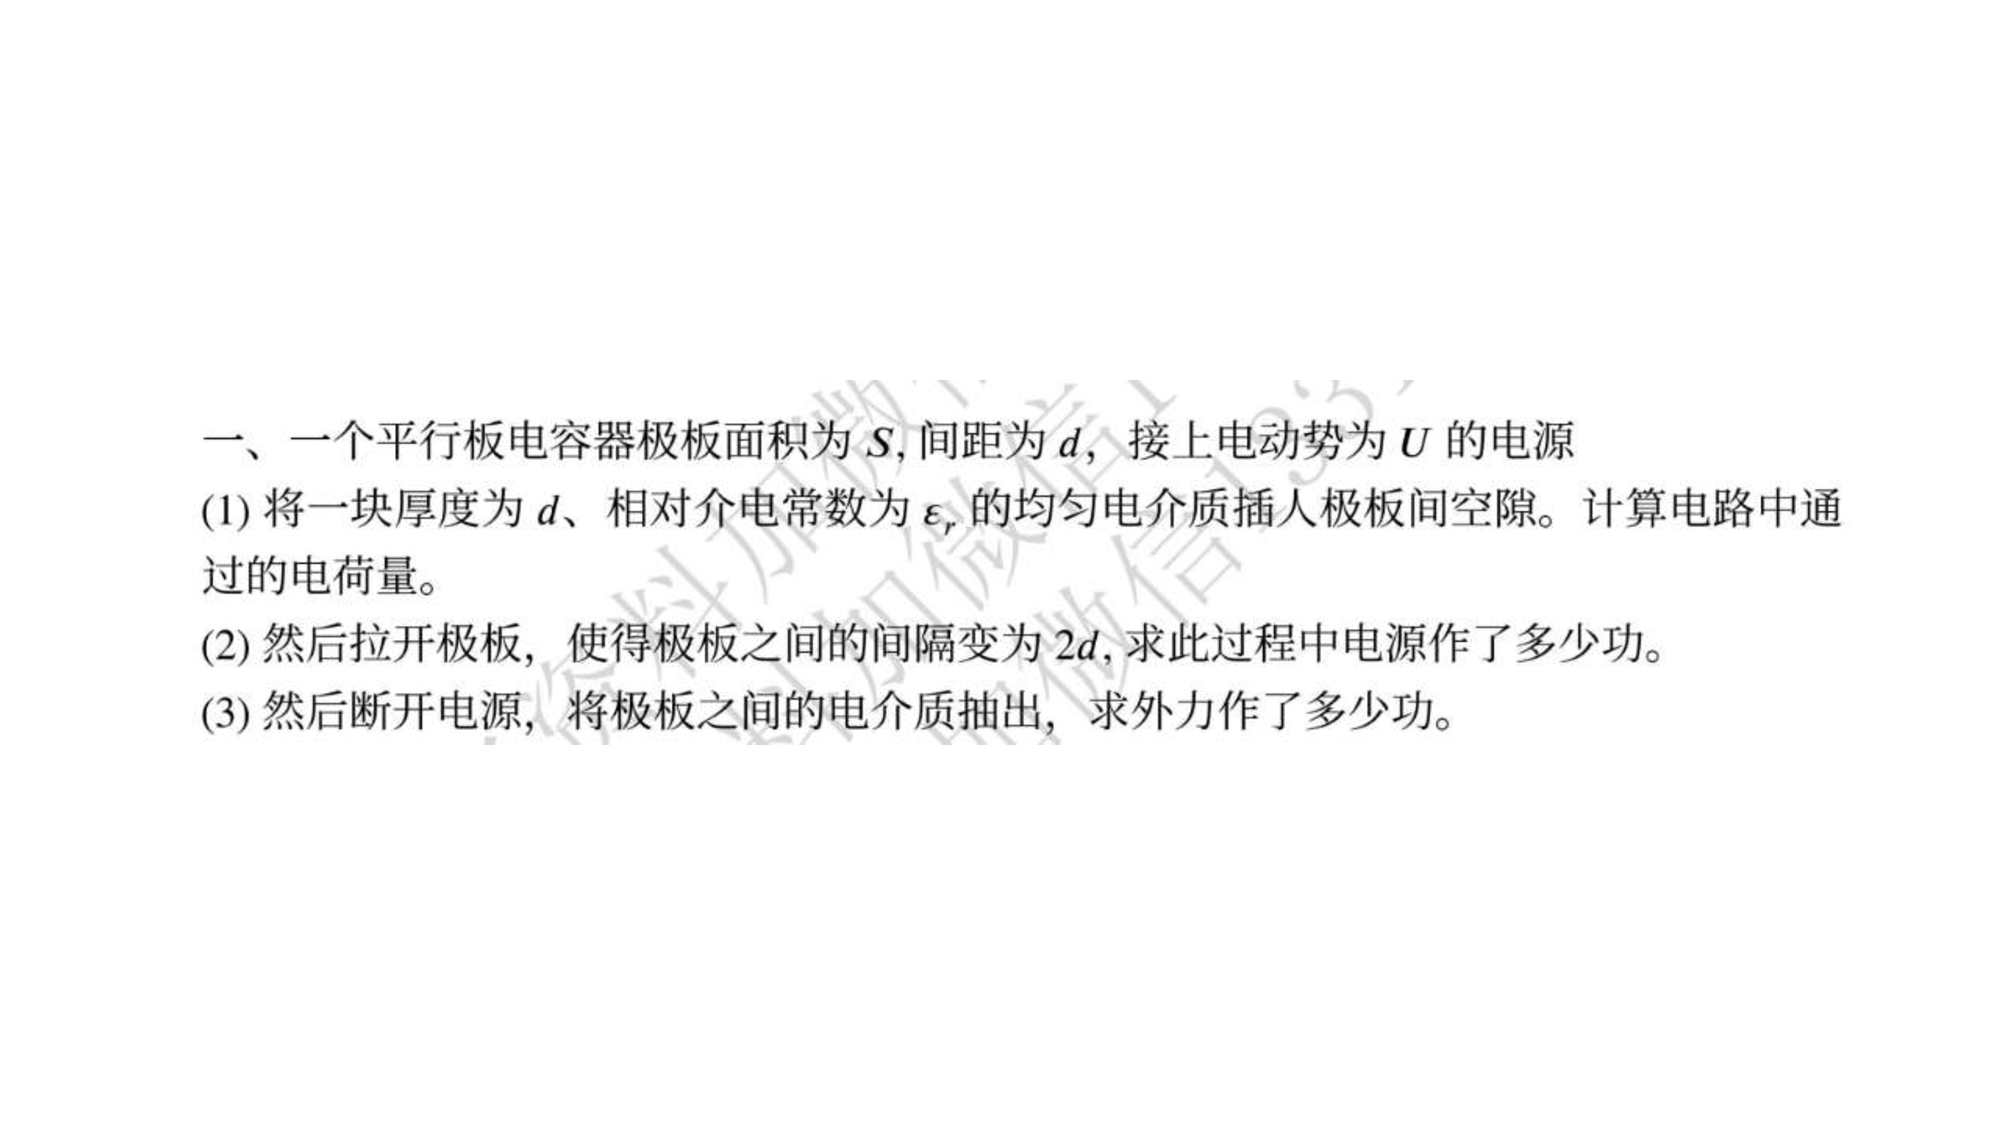
\includepdf[pages=-]{习题.pdf}
%\section{附录B:本学期作业合集}
%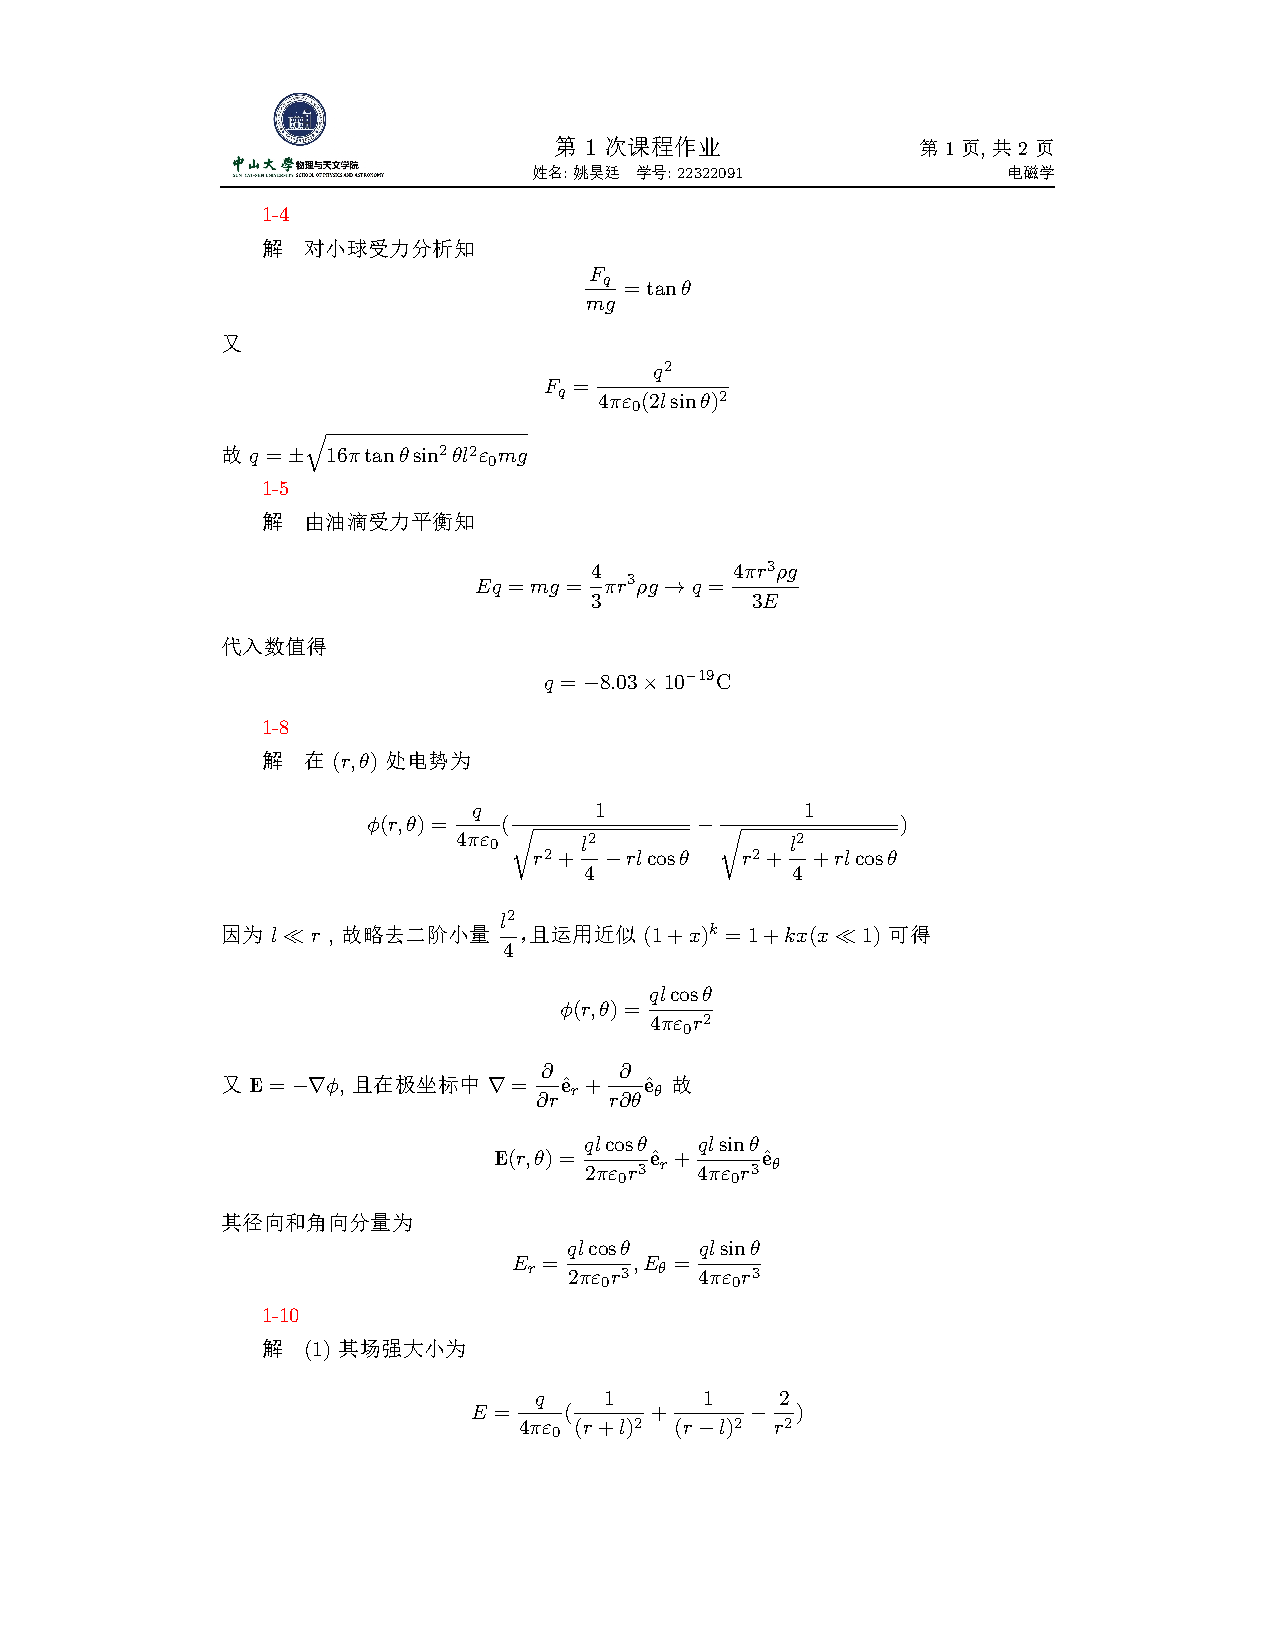
\includepdf[pages=-]{作业合集.pdf}
\end{document}